\documentclass[9pt]{extarticle}
\usepackage{spconf,amsmath,graphicx}
\usepackage{algorithm}
\usepackage{algpseudocode}
\usepackage{amssymb}
\usepackage{amsthm}
\usepackage{xcolor}
\usepackage{caption}
\captionsetup{font=small, labelfont=bf}
\usepackage{enumitem}
\usepackage{hyperref}
\newtheorem{theorem}{Theorem}
\newtheorem{lemma}{Lemma}
\newtheorem{proposition}{Proposition}
\newtheorem{corollary}{Corollary}
\newtheorem{assumption}{Assumption}
 % smaller font inside algorithms
\makeatother
\algrenewcommand\algorithmicrequire{\textbf{In:}}
\algrenewcommand\algorithmicensure{\textbf{Out:}}
\algrenewcommand\algorithmicindent{0.8em}
\newcommand{\dk}[1]{\textbf{\textcolor{red}{ {DK: #1}}}}
\theoremstyle{definition}
\newtheorem{definition}[theorem]{Definition}
\newtheorem{example}[theorem]{Example}
\newtheorem{remark}[theorem]{Remark}
\newtheorem{notation}[theorem]{Notation}
% Notation convenience (optional)
\newcommand{\hadam}{\circ}
\newcommand{\ones}{\mathbf{1}}
\allowdisplaybreaks
% spconf.sty's \@sect override has no run-in branch, so the standard \paragraph
% errors (undefined \@svsechd); use a plain unnumbered run-in heading instead.
\renewcommand{\paragraph}[1]{\par\medskip\noindent{\bf #1}\hspace{0.5em}\ignorespaces}
\hyphenation{op-tical net-works semi-conduc-tor}
\begin{document}
\title{Optimally Transport Weighted Stochastic Gradient Descent to Mitigate Distribution Shift\vspace{-8pt}}
% make the title area
\maketitle

\begin{abstract}
Stochastic gradient descent implicitly assumes that mini-batches are exchangeable draws from a fixed population, but real datasets are often organized into critical groups, such as demographic categories, recording sites, or data sources, whose relative importance in the objective may need to be set explicitly rather than inherited from raw sample counts. This is straightforward when every group can appear in every batch; it breaks down when batches can only reveal a subset of groups at a time, which is the rule rather than the exception whenever collection logistics, storage layout, or access constraints determine which groups can co-occur. Naive fixes, such as fixed reweighting or oversampling, either ignore which groups a given batch can actually show or inflate variance and discard data. We propose a fair stochastic gradient descent framework that treats per-batch reweighting as a masked optimal transport problem, coupling the distribution over observable batch patterns to a target group distribution through a support mask determined by which groups can co-occur. Solving this transport problem yields per-batch weights that make the resulting stochastic gradient exactly unbiased for the target objective whenever a feasible transport plan exists, and a classical max-flow/min-cut feasibility condition, specialized to our masked setting, characterizes exactly when it does. We show the resulting projected algorithm converges at the standard rate for convex objectives, and that when exact feasibility fails, an entropy-regularized projection recovers the closest achievable target distribution together with an explicit, controllable bound on the resulting bias. We validate the approach, instantiated as FedAVOT, on income classification with demographic fairness metrics and on age regression under a realistic mismatch between how often a group is observable and how much it should count, where it tracks full-coverage performance whenever the underlying transport problem is feasible, improves on the uniform batch average by a margin that a closed-form feasibility diagnostic predicts before training, and remains stable in regimes where the standard fixed-multiplier correction diverges.
\end{abstract}

\section{Introduction}

Empirical risk minimization treats every training example as interchangeable, but many datasets carry group structure that the learner is expected to respect: demographic attributes in fairness-sensitive applications, subject or site identity in clinical and scientific data, device or sensor type in heterogeneous sensing, or domain label in multi-source data. When the objective is meant to weight these groups according to some target distribution, for instance uniformly across demographic groups regardless of their prevalence in the data, the standard fix is to reweight the loss or resample the data so that the empirical group frequencies match the target. This works cleanly when a mini-batch can, in principle, contain any group; the reweighting reduces to a fixed multiplier per group.

That assumption fails whenever batches are constrained to show only a subset of groups at a time. Streaming pipelines with bounded buffers deliver whichever groups happen to be resident; sensor and measurement networks return data only from the sites reachable at that moment; records held under access or privacy restrictions can be read only in permitted combinations; and in any pipeline where a batch is assembled from a few sources at a time, the batch is by construction restricted to whichever groups those sources carry. In these settings, a fixed per-group multiplier is not well defined, because the same group can appear alongside different partners from one iteration to the next, and some target distributions may not be achievable at all under the batch structure actually realized. Existing remedies do not resolve this: importance-sampling and variance-reduction methods for SGD assume itemwise access rather than subset-masked batches, distributionally robust and fairness-reweighting methods operate on the objective rather than on the batch-level aggregation constraint, and methods that correct for a known per-group observation rate assume a fixed correction factor rather than one that adapts to which combinations of groups can jointly appear.

We address this by casting per-batch reweighting as a transport problem: probability mass must move from the distribution over observable batch patterns to the desired target distribution over groups, subject to a combinatorial mask that only allows mass to flow between a batch pattern and the groups it actually contains. Unlike classical optimal transport, there is no cost to minimize; the only question is feasibility, which admits a clean max-flow/min-cut characterization obtained by specializing classical flow-feasibility results~\cite{fordfulkerson1962flows,hall1935representatives} to the batch-sampling mask. When feasible, the resulting transport plan gives per-batch weights that make the stochastic gradient exactly unbiased for the target objective, and we prove the associated projected SGD algorithm converges at the standard $O(1/\sqrt{T})$ rate for convex objectives. When infeasible, for instance, because certain groups never co-occur in a batch, we show that an entropy-regularized projection still returns a well-defined, feasible surrogate target distribution, and we bound the resulting suboptimality by the same convergence rate plus an explicit, tunable bias term governed by how far the surrogate had to move from the intended target.

We instantiate this framework as FedAVOT and evaluate it in two settings: fairness-sensitive classification on the Adult income dataset under a uniform importance target across race, and age regression on IMDb-Wiki under a realistic availability mismatch, where the groups most important to the target objective are not the ones most likely to be observed. Across both, FedAVOT tracks the full-coverage objective whenever the transport problem is feasible, improves on the uniform batch average throughout the infeasible range short of support collapse, with a margin that a closed-form floor computed from the transport plan alone predicts before training, and remains stable in regimes where the fixed-multiplier correction, which presumes a uniform observation rate, diverges. We summarize our contributions below.

\subsection*{Related work}
\paragraph{SGD, importance sampling, and variance reduction.}
A large literature improves SGD via adaptive or importance sampling to reduce variance or accelerate convergence (e.g., non-uniform sampling by Lipschitz constants or gradient magnitudes). These methods typically assume \emph{itemwise} access and do not handle \emph{subset-masked} batching constraints, making their unbiasedness/variance guarantees fragile when groups appear jointly or not at all in a mini-batch. See, e.g., importance sampling for SGD and mini-batches~\cite{needell2016sgd,alain2015variance,csiba2018minibatch}, OT-based variance reduction~\cite{blanchet2023optimal}, and broad surveys of large-scale optimization~\cite{bottou2018optimization}.
\paragraph{Class imbalance, fairness, and group-robust learning.}
Oversampling/undersampling and static reweighting are standard in class imbalance, but they inflate variance or discard data. Group distributionally robust optimization (GroupDRO) directly optimizes worst-group risk via (sub)gradient methods~\cite{sagawa2020distributionally}, while other fairness-aware reweighting schemes adapt group weights during training. These approaches act at the objective level but do not address \emph{subset-induced masking} during gradient aggregation; our construction guarantees unbiasedness \emph{per batch} under the mask by solving a structured coupling.
\paragraph{Domain adaptation and covariate shift.}
Importance weighting for covariate shift seeks to correct training-test mismatch by density-ratio reweighting~\cite{sugiyama2008covariate}. OT-based domain adaptation transports mass between source and target distributions~\cite{courty2017optimal}. Our use of OT differs: we do not move samples in feature space; instead, we \emph{transport mass between subset events and groups} under a combinatorial mask to produce unbiased per-batch weights consistent with a prescribed target mixture $p$.
\paragraph{Subset-observable batches and group heterogeneity.}
The setting in which a batch exposes only a few groups at a time has been studied most systematically in distributed learning, where the groups are data-holding sources and only a sampled few report at a time. Canonical methods there (FedAvg, FedProx, SCAFFOLD, q-FFL) address drift, stability, or fairness via objective regularization, control variates, or global reweighting~\cite{mcmahan2017communication,li2020fedprox,karimireddy2020scaffold,li2020qffl}, and the agnostic formulation optimizes against an adversarial mixture over groups~\cite{mohri2019agnostic}. Our method is complementary and not tied to that architecture: it prescribes \emph{per-iteration transport weights} matching a target group mixture even when batches reveal only a subset of groups, and it quantifies feasibility limits via masked OT (with principled relaxations in the unbalanced regime).
\paragraph{Inverse-propensity (Horvitz--Thompson) reweighting.}
The classical alternative to transport weights is inverse-propensity weighting: weight each observed group by $p_i/\pi_i$, where $\pi_i$ is its inclusion probability, which yields an unbiased gradient estimator whenever $\pi_i > 0$~\cite{horvitz1952generalization}, even when the transport problem is infeasible. The cost is variance, and the two approaches part company exactly at our feasibility condition: since $p_i \le \pi_i$ is the same statement as $p_i/\pi_i \le 1$, the inverse-propensity correction exceeds unity precisely on the groups for which the transport problem is infeasible, i.e., in the regime where reweighting matters most. How damaging that is depends on the magnitude of the ratio and on whether the loss is bounded: mild excesses are tolerable, while the fixed $m/K$ correction of Section~\ref{sec:experiments}, applied under availability-aligned sampling to an unbounded quadratic loss, amplifies the iterates until they diverge. FedAVOT sits at the other end of the tradeoff: its per-batch weights are convex combinations by construction, so the iterates remain stable for any mask, at the price of a bias that is zero when the transport is feasible and explicitly bounded via $\|p-\hat{p}\|_1$ when it is not (Section~\ref{subsec:infeasible}). The relevant comparison is thus stability versus bias, not unbiasedness alone.
\paragraph{Masked / constrained OT and generalized Sinkhorn.}
Capacity and support constraints in OT have been studied via linear constraints and Bregman-projection algorithms~\cite{benamou2015iterative,chizat2018scaling,korman2015capacity}. We leverage these tools to (i) certify feasibility via flow-cut conditions and (ii) compute couplings with masking efficiently. In infeasible cases, unbalanced/divergence-penalized OT~\cite{chizat2018scaling,liero2018optimal} provides a controlled projection from $p$ onto feasible marginals $\hat{p}$, preserving algorithmic scalability.
\subsection*{Contributions}
\begin{enumerate}
\item \textbf{Transport-weighted SGD under subset masking.} We formulate per-batch gradient aggregation as a masked OT feasibility problem coupling the subset law $q$ and target mixture $p$; the resulting weights ensure \emph{per-iteration} unbiasedness for $F_p$ when feasible.
\item \textbf{General feasibility and projection in the infeasible regime.} Specializing a classical flow-feasibility condition to the batch-sampling mask, we delineate when exact alignment is impossible (missing co-occurrences, sparse exposure of critical groups), show that entropy/Bregman-regularized scaling returns a feasible $\hat{p}$, and derive an explicit $O(T^{-1/2})+O(\|p-\hat{p}\|)$ performance bound.
\item \textbf{Convergence theory with projection.} For convex objectives on a compact set, transport-weighted projected SGD enjoys the classical $\mathcal{O}(T^{-1/2})$ rate; we give a modular proof that cleanly separates optimization error from marginal-mismatch bias.
\item \textbf{Algorithmic framework.} We provide a masked Sinkhorn/IPFP routine (and generalized unbalanced variants) that scales to many groups/subsets and integrates seamlessly with standard SGD codepaths.
\end{enumerate}
Overall, our results turn subset-masked batching from a liability into a design lever: by computing transport weights that respect what a batch \emph{can} show and aligning them to what the objective \emph{should} emphasize, we obtain principled, scalable, and distributionally aligned SGD.
\section{Transport-Weighted SGD with Subset Sampling: Setup and Convergence}
We begin by formalizing the optimization setup, followed by the probabilistic and geometric interpretation of the proposed transport-weighted sampling procedure. Our goal is to provide a unifying view of mini-batch sampling and fairness weighting through a transport-theoretic lens.

Consider a general regression problem where the feature space is $\mathcal{X}\subset \mathbb{R}^d$, the target space is $\mathcal{Y}\subset \mathbb{R}$, and the model class is $\mathcal{F}=\{f_\theta:\mathcal{X}\rightarrow \mathcal{Y}\mid \theta\in\Theta\}$ with parameters $\theta\in\Theta$. Let $\ell:\mathcal{Y}\times\mathcal{Y}\rightarrow \mathbb{R}_+$ denote a loss function (e.g., squared loss $\ell(a,b)=(a-b)^2$). Given a dataset $\{(x_i,y_i)\}_{i=1}^N$, the standard empirical risk minimization (ERM) objective is:
\begin{equation}\label{eq:erm}
\boxed{\min_{\theta\in\Theta} \ \frac{1}{N}\sum_{i=1}^{N}\ell(f_\theta(x_i),y_i)}.
\end{equation}

In many practical settings, the data exhibit distinct \emph{critical groups}, such as demographic categories, device types, or environments, which we denote by $\mathcal{K}=\{K_1,\ldots,K_m\}$, where each $K_j\subset\mathcal{X}$ is a partition of the feature space. Each datapoint $x_i$ belongs to exactly one critical group $K_j$.
Let $N_j$ be the number of samples belonging to group $K_j$, so that $\sum_{j=1}^m N_j = N$. Then the ERM objective~\eqref{eq:erm} can be rewritten as a weighted sum over these subgroups:
\begin{equation}\label{eq:erm-groups}
\boxed{\min_{\theta\in\Theta} \ \sum_{j=1}^{m}\frac{N_j}{N}\left(\frac{1}{N_j}\sum_{(x_i,y_i)\in K_j}\ell(f_\theta(x_i),y_i)\right)}.
\end{equation}
Here, $\frac{N_j}{N}$ is the empirical marginal probability of group $j$, denoted by $\nu_j$. The resulting empirical measure $\hat{\nu}=(\nu_1,\ldots,\nu_m)$ may be \emph{imbalanced}, e.g., $\nu_1\gg\nu_2$, leading to biased training toward majority groups.
\paragraph{Example.}
Suppose a dataset consists of $N_1=900$ and $N_2=100$ samples from two demographic groups. Then the ERM objective gives weights $(\nu_1,\nu_2)=(0.9,0.1)$. If we desire fairness or robustness, we may wish to train under a target distribution $\mu=(0.5,0.5)$ that equalizes importance across groups.

To correct this imbalance, we define a \emph{target group measure} $\mu=(\mu_1,\ldots,\mu_m)$ over $\mathcal{K}$, representing the desired weighting (e.g., uniform or risk-adjusted). The corresponding fair optimization objective becomes:
\begin{equation}\label{eq:fair-obj}
\boxed{\min_{\theta\in \Theta}\ \sum_{j=1}^{m}\mu_j\,\mathbb{E}_{(x,y)\in K_j}\left[\ell(f_\theta(x),y)\right]}.
\end{equation}
When $\mu=\nu$, this reduces to standard ERM; otherwise, it enforces fairness or domain alignment by up/down-weighting subgroups. Naïve oversampling or undersampling approximates this by modifying the data distribution, but these techniques may increase variance or discard data~\cite{buda2018systematic, he2009learning}.

In practice, optimization proceeds via stochastic gradient descent (SGD). At iteration $t$, a random subset (mini-batch) $\xi_t\subset\{1,\ldots,N\}$ is drawn \emph{without replacement}. Let $\mathcal{A}_1,\ldots,\mathcal{A}_{2^m-1}$ denote all non-empty subsets of $\mathcal{K}$ that may appear in a batch, and let $q_j$ be the probability that the active batch at iteration $t$ contains exactly the subgroup pattern $\mathcal{A}_j$.
For example, with $m=2$ groups, there are three possible subset categories:
\[
\mathcal{A}_1=\{K_1\},\quad \mathcal{A}_2=\{K_2\},\quad \mathcal{A}_3=\{K_1,K_2\},
\]
with associated probabilities $(q_1,q_2,q_3)$ depending on the sampling process. Throughout the analysis we treat $q$ as known; when it is not available in closed form, it can be estimated offline by Monte Carlo simulation of the batch sampler, which is how our experiments obtain it (Section~\ref{sec:experiments}).
\paragraph{Weighted Gradient Aggregation.}
When the mini-batch $\xi_t$ belongs to $\mathcal{A}_j$, each group $i\in\mathcal{A}_j$ contributes a normalized proportion $Y[i,j]$ to the aggregated gradient. The joint allocation of group mass is given by:
\[
T[i,j] = q_j\,Y[i,j],
\]
representing the amount of probability mass transported from event $j$ (subset $\mathcal{A}_j$) to group $i$.

The weight assignment must satisfy:
\begin{align}\label{eq:constraints}
    &\sum_{j}T[i,j]=p_i=\mu_i, && \forall i, \nonumber\\
    &\sum_{i}T[i,j]=q_j, && \forall j, \nonumber\\
    &T[i,j]=0, && i\notin\mathcal{A}_j, \nonumber\\
    &T[i,j]\ge0, && \forall (i,j),
\end{align}
where the support mask $\mathcal{E}=\{(i,j)\mid i\in\mathcal{A}_j\}$ enforces feasible interactions between groups and subset events. These are exactly the marginal and non-negativity constraints of a \emph{masked optimal transport (MOT)} problem:
\begin{equation}\label{eq:mot}
T\mathbf{1}_M=p, \quad \mathbf{1}_N^\top T=q, \quad T\ge0, \quad \operatorname{supp}(T)\subseteq \mathcal{E}.
\end{equation}
Unlike classical OT~\cite{villani2009optimal, peyre2019computational}, we do not minimize a transport \emph{cost}; feasibility alone suffices, as long as mass can be transferred from $q$ to $p$ under the mask. The corresponding Kantorovich relaxation~\cite{kantorovich1942transfer} reads:
\begin{equation}\label{eq:kantorovich}
\min_{T\ge0}\sum_{i,j}C[i,j]T[i,j]\quad\text{s.t.}\quad T\mathbf{1}_M=p,\;\mathbf{1}_N^\top T=q,
\end{equation}
where
\[
C[i,j] =
\begin{cases}
1, & \text{if } i\in\mathcal{A}_j,\\
\infty, & \text{otherwise.}
\end{cases}
\]

Feasibility of~\eqref{eq:mot} admits a simple max-flow/min-cut characterization: the following theorem specializes the classical supply--demand feasibility theorem of Ford and Fulkerson~\cite{fordfulkerson1962flows}, whose bipartite ancestor is Hall's marriage theorem~\cite{hall1935representatives}, to the membership mask $\mathcal{E}$.
\begin{theorem}[\textbf{Feasibility of Masked OT}~\cite{fordfulkerson1962flows,hall1935representatives}]
\label{thm:feasibility}
Let $I\subseteq[N]$, $\mathcal{N}(I):=\{j\mid \exists i\in I,\ (i,j)\in\mathcal{E}\}$, and $\mathcal{S}(I):=\{j\mid \mathcal{A}_j\subseteq I\}$. Then~\eqref{eq:mot} is feasible iff
\begin{equation}\label{eq:feasibility}
\sum_{j\in\mathcal{S}(I)} q_j \le \sum_{i\in I} p_i \le \sum_{j\in\mathcal{N}(I)} q_j, \quad \forall I\subseteq[N].
\end{equation}
\end{theorem}
\paragraph{Example.}
For two groups with $\mu=(0.5,0.5)$ and $(q_1,q_2,q_3)=(0.2,0.2,0.6)$, the feasibility inequalities reduce to:
\[
q_1 \le \mu_1 \le q_1+q_3,\quad q_2 \le \mu_2 \le q_2+q_3,
\]
which are satisfied, so a feasible transport $T$ exists.

Given feasibility, $T$ can be computed efficiently using the \textit{Iterative Proportional Fitting Procedure (IPFP)}~\cite{sinkhorn1967concerning, knight2008sinkhorn}, also known as \textit{Sinkhorn scaling}, which alternates between row and column normalization.
\begin{algorithm}[h]
\caption{Sinkhorn Scaling for Masked Transport Map}
\label{alg:sinkhorn}
\begin{algorithmic}[1]
\Require $p,q,\mathcal{E},\varepsilon$
\State Initialize $T^{(0)}\ge0$ with $\operatorname{supp}(T^{(0)})\subseteq\mathcal{E}$, $T^{(0)\top}\mathbf{1}=q$
\For{$t=0,1,2,\ldots$}
  \State $r \gets p \oslash (T^{(t)}\mathbf{1})$; \quad $\tilde T \gets \operatorname{Diag}(r)\,T^{(t)}$
  \State $c \gets q \oslash (\tilde T^\top\mathbf{1})$; \quad $T^{(t+1)} \gets \tilde T\,\operatorname{Diag}(c)$
  \If{$\|T^{(t+1)}\mathbf{1}-p\|_1 \le \varepsilon$ and $\|\mathbf{1}^\top T^{(t+1)}-q^\top\|_1 \le \varepsilon$} \textbf{stop}
  \EndIf
\EndFor
\State \Return $T^{(t+1)}$, normalized weights $Y \gets T^{(t+1)}\,\mathrm{Diag}(q)^{-1}$
\end{algorithmic}
\end{algorithm}
\begin{theorem}[\textbf{Convergence of IPFP}~\cite{sinkhorn1967concerning, knight2008sinkhorn}]
\label{thm:ipfp}
If $p$ and $q$ satisfy~\eqref{eq:feasibility}, Algorithm~\ref{alg:sinkhorn} with $\varepsilon=0$ converges to a feasible solution of~\eqref{eq:mot}.
\end{theorem}

Entropy-regularized variants~\cite{cuturi2013sinkhorn} guarantee convergence to a unique minimizer of an entropy-augmented objective:
\[
\min_{T\ge0} \sum_{i,j}C[i,j]T[i,j]+\varepsilon \sum_{i,j}T[i,j]\log T[i,j],
\]
whose dual corresponds to coordinate ascent in the log-domain~\cite{csiszar1975ipr}. Practically, this allows soft transport assignments and numerically stable convergence.
In mini-batch training, given a batch $\xi_t$ consisting of $n_1$ samples from group $1$ and $n_2$ samples from group $2$, the transport plan yields weights:
\[
w_1 = T[1,\{1,2\}], \quad w_2 = T[2,\{1,2\}],
\]
and we scale per-sample gradients accordingly. This ensures each SGD step is proportionally weighted according to the global target distribution $\mu$, while respecting the random subset structure induced by $\xi_t$.
\section{Convergence of Projected Transport-Weighted SGD (FedAVOT)}
We analyze the projected SGD algorithm that uses the transport weights described earlier to produce an unbiased stochastic gradient of the \emph{target} (fair) objective
\begin{equation}\label{eq:target-objective}
F(\theta) \;:=\; \sum_{i=1}^m \mu_i \,\mathbb{E}_{(x,y)\sim \mathcal{D}_i}\!\big[\ell\!\left(f_\theta(x),y\right)\big],
\qquad \theta\in\Theta,
\end{equation}
where $\mathcal{D}_i$ is the (unknown) data distribution within group $K_i$ and $(\mu_1,\dots,\mu_m)$ is the desired target measure over groups. We assume $F$ is convex on a nonempty, closed, convex, and compact constraint set $\mathcal{C}\subseteq\Theta$; the projection $\Pi_{\mathcal{C}}$ is therefore well-defined. Let $\theta^\star\in\arg\min_{\theta\in\mathcal{C}}F(\theta)$.
\paragraph{Sampling and weighting.}
At iteration $t$, a mini-batch $\xi_t$ is drawn (without replacement) from the dataset; let $j_t\in\{1,\dots,M\}$ index the \emph{active group-subset} $\mathcal{A}_{j_t}\subseteq\{1,\dots,m\}$ observed in that batch. As in the setup, let $q_j=\mathbb{P}(j_t=j)$ be the probability of subset $\mathcal{A}_j$ under the sampling scheme, and let $Y[i,j]\ge 0$ denote the normalized contribution (weight) assigned to group $i$ when the active subset is $j$ (so $Y[i,j]=0$ if $i\notin\mathcal{A}_j$). Define $T[i,j]=q_j Y[i,j]$ and recall the masking and marginal constraints
\begin{equation}\label{eq:marginals}
\sum_{j=1}^M T[i,j]=\mu_i,\quad \sum_{i=1}^m T[i,j]=q_j,\quad T[i,j]=0 \ \text{if}\ i\notin\mathcal{A}_j.
\end{equation}
Hence $\sum_{j} q_j Y[i,j]=\mu_i$ for all $i$.
Within batch $\xi_t$, we compute the (per-sample) gradients and aggregate them group-wise, then scale by the transport weights so that the stochastic gradient estimator is
\begin{equation}\label{eq:gt}
g_t \;=\; \sum_{i\in\mathcal{A}_{j_t}} Y[i,j_t]\;\widehat{g}_{t,i},
\qquad
\text{with}\quad
\widehat{g}_{t,i} \;=\; \frac{1}{|\xi_t\cap K_i|}\sum_{(x,y)\in \xi_t\cap K_i} \nabla_\theta \ell\!\left(f_{\theta_t}(x),y\right).
\end{equation}
(When $|\xi_t\cap K_i|=0$, we interpret $\widehat{g}_{t,i}$ as $0$ and $Y[i,j_t]=0$ by construction.)
\begin{assumption}[\textbf{Bounded second moment}]\label{assump:gradient_bound}
There exists $G>0$ such that for all $\theta\in\mathcal{C}$,
\[
\mathbb{E}\!\left[\|g_t\|^2 \,\big|\, \theta_t=\theta\right] \;\le\; G^2.
\]
\end{assumption}
\noindent
Compactness of $\mathcal{C}$ and local Lipschitz continuity of $\nabla \ell\!\left(f_\theta(\cdot),\cdot\right)$ on $\mathcal{C}$ (induced by convexity of $F$ on $\mathcal{C}$) together with the bounded mini-batch size imply Assumption~\ref{assump:gradient_bound} under standard conditions; alternatively, one may assume a uniform bound on per-sample gradient norms on $\mathcal{C}$.
\begin{lemma}[\textbf{Unbiasedness}]\label{lem:unbiased}
Under \eqref{eq:marginals}, the estimator $g_t$ in \eqref{eq:gt} is conditionally unbiased:
\[
\mathbb{E}\!\left[g_t \,\big|\, \theta_t\right] \;=\; \nabla F(\theta_t).
\]
\end{lemma}
\begin{proof}
Condition on $\theta_t$. For each group $i$, the within-group batch average satisfies
$\mathbb{E}\big[\widehat{g}_{t,i}\,\big|\,\theta_t,i\in\mathcal{A}_{j_t}\big]=\mathbb{E}_{(x,y)\sim\mathcal{D}_i}\big[\nabla_\theta \ell(f_{\theta_t}(x),y)\big]$.
Taking expectation over the subset index $j_t$ yields
\begin{multline}
\mathbb{E}[g_t\mid \theta_t]
= \sum_{j=1}^M q_j \sum_{i\in\mathcal{A}_j} Y[i,j]\;\mathbb{E}_{(x,y)\sim\mathcal{D}_i}\!\big[\nabla_\theta \ell(f_{\theta_t}(x),y)\big]
\\= \sum_{i=1}^m \left(\sum_{j=1}^M q_j Y[i,j]\right)\, \mathbb{E}_{\mathcal{D}_i}\!\big[\nabla_\theta \ell(f_{\theta_t}(x),y)\big].
\end{multline}
Using $\sum_j q_j Y[i,j]=\mu_i$ gives
$$\mathbb{E}[g_t\mid \theta_t] = \sum_{i=1}^m \mu_i\, \mathbb{E}_{\mathcal{D}_i}\!\big[\nabla_\theta \ell(f_{\theta_t}(x),y)\big] = \nabla F(\theta_t),$$ which proves the claim.
\end{proof}
\subsection{Algorithm}
\begin{algorithm}[H]
\caption{\textsc{Projected Transport-Weighted SGD} (FedAVOT)}
\label{alg:fedavot}
\begin{algorithmic}[1]
\Require Initial point $\theta_1\in\mathcal{C}$, step sizes $\{\eta_t\}_{t=1}^T$, target marginals $p=\mu$, subset probabilities $q$, mask $\mathcal{E}$, tolerance $\varepsilon$
\State Precompute (or update online) a feasible transport plan $T$ via Sinkhorn/IPFP on the mask $\mathcal{E}$ so that $T\mathbf{1}=p$ and $\mathbf{1}^\top T=q^\top$
\State Set $Y \gets T\,\mathrm{Diag}(q)^{-1}$ \Comment{Normalized per-subset group weights}
\For{$t=1$ to $T$}
    \State Sample a mini-batch $\xi_t$ (without replacement) and identify active group-subset $j_t$ with $\mathcal{A}_{j_t}$
    \State For each $i\in\mathcal{A}_{j_t}$, compute $\widehat{g}_{t,i}=\frac{1}{|\xi_t\cap K_i|}\sum_{(x,y)\in\xi_t\cap K_i} \nabla_\theta \ell(f_{\theta_t}(x),y)$
    \State Form the weighted gradient $g_t = \sum_{i\in\mathcal{A}_{j_t}} Y[i,j_t]\;\widehat{g}_{t,i}$
    \State Update $\theta_{t+1} \gets \Pi_{\mathcal{C}}\!\big(\theta_t - \eta_t g_t\big)$
\EndFor
\State \Return either the average iterate $\bar{\theta}_T=\frac{1}{T}\sum_{t=1}^T \theta_t$ or the best-so-far iterate
\end{algorithmic}
\end{algorithm}
\subsection{Convergence Rate}
Let $D:=\sup_{\theta,\theta'\in\mathcal{C}}\|\theta-\theta'\|$ denote the (finite) diameter of $\mathcal{C}$ in the Euclidean norm. Consider the averaged iterate $\bar{\theta}_T := \frac{1}{T}\sum_{t=1}^T \theta_t$.
\begin{theorem}[\textbf{Projected FedAVOT: $O(1/\sqrt{T})$ suboptimality}]\label{thm:main}
Suppose $F$ is convex on $\mathcal{C}$, Assumption~\ref{assump:gradient_bound} holds, and the gradient estimator $g_t$ is unbiased (Lemma~\ref{lem:unbiased}). For any step sizes $\{\eta_t\}_{t=1}^T$,
\begin{equation}\label{eq:key-bound}
\mathbb{E}\!\left[F(\bar{\theta}_T) - F(\theta^\star)\right]
\;\le\;
\frac{\|\theta_1-\theta^\star\|^2}{2\sum_{t=1}^T \eta_t}
\;+\;
\frac{G^2}{2T}\sum_{t=1}^T \eta_t.
\end{equation}
In particular, with the choice $\eta_t \equiv \eta = \frac{D}{G\sqrt{T}}$,
\begin{equation}\label{eq:rate}
\mathbb{E}\!\left[F(\bar{\theta}_T) - F(\theta^\star)\right]
\;\le\; \frac{DG}{\sqrt{T}}.
\end{equation}
\end{theorem}
\begin{proof}
Let $\theta^\star\in\arg\min_{\mathcal{C}} F$. By non-expansiveness of the Euclidean projection and the update $\theta_{t+1}=\Pi_{\mathcal{C}}(\theta_t-\eta_t g_t)$,
\begin{align*}
\|\theta_{t+1}-\theta^\star\|^2
&\le \|\theta_t-\eta_t g_t - \theta^\star\|^2
= \|\theta_t-\theta^\star\|^2 - 2\eta_t \langle g_t,\, \theta_t-\theta^\star\rangle + \eta_t^2 \|g_t\|^2.
\end{align*}
Taking conditional expectation given $\theta_t$ and using Lemma~\ref{lem:unbiased},
\[
\mathbb{E}\!\left[\|\theta_{t+1}-\theta^\star\|^2 \,\big|\, \theta_t\right]
\le
\|\theta_t-\theta^\star\|^2 - 2\eta_t \langle \nabla F(\theta_t),\, \theta_t-\theta^\star\rangle + \eta_t^2\,\mathbb{E}\!\left[\|g_t\|^2 \mid \theta_t\right].
\]
By convexity, $F(\theta_t)-F(\theta^\star)\le \langle \nabla F(\theta_t), \theta_t-\theta^\star\rangle$. Applying Assumption~\ref{assump:gradient_bound} and then total expectation,
\[
\mathbb{E}\!\left[\|\theta_{t+1}-\theta^\star\|^2\right]
\le
\mathbb{E}\!\left[\|\theta_t-\theta^\star\|^2\right]
- 2\eta_t\, \mathbb{E}\!\left[F(\theta_t)-F(\theta^\star)\right]
+ \eta_t^2 G^2.
\]
Summing over $t=1,\dots,T$ and telescoping,
\[
2\sum_{t=1}^T \eta_t \,\mathbb{E}\!\left[F(\theta_t)-F(\theta^\star)\right]
\;\le\;
\|\theta_1-\theta^\star\|^2 - \mathbb{E}\!\left[\|\theta_{T+1}-\theta^\star\|^2\right] + G^2 \sum_{t=1}^T \eta_t^2
\;\le\;
\|\theta_1-\theta^\star\|^2 + G^2 \sum_{t=1}^T \eta_t^2.
\]
By convexity of $F$ and Jensen’s inequality,
\[
\mathbb{E}\!\left[F(\bar{\theta}_T)\right]
\le \frac{1}{T}\sum_{t=1}^T \mathbb{E}\!\left[F(\theta_t)\right].
\]
Combining the last two displays and dividing by $2\sum_{t=1}^T\eta_t$ gives \eqref{eq:key-bound}. For the constant steps $\eta_t\equiv\eta$, choose $\eta=\frac{D}{G\sqrt{T}}$; use $\|\theta_1-\theta^\star\|\le D$ and $\sum_{t=1}^T \eta_t = T\eta$, $\sum_{t=1}^T \eta_t^2=T\eta^2$ to obtain
\[
\frac{D^2}{2T\eta}+\frac{G^2}{2}\eta \;=\; \frac{D^2}{2T}\frac{G\sqrt{T}}{D} + \frac{G^2}{2}\frac{D}{G\sqrt{T}} \;=\; \frac{DG}{\sqrt{T}},
\]
which establishes \eqref{eq:rate}.
\end{proof}
\begin{remark}[On choices of stepsizes]
The bound \eqref{eq:key-bound} also yields the classical $O(1/\sqrt{T})$ rate when using $\eta_t = \eta_0/\sqrt{t}$ (up to constants). The constant $DG$ reflects the geometry (diameter) of $\mathcal{C}$ and the second-moment bound of the transport-weighted gradient estimator.
\end{remark}
\begin{remark}[Effect of transport reweighting]
The masked-OT reweighting controls the \emph{bias} of the stochastic gradient by enforcing the marginal constraints \eqref{eq:marginals}. Under the same mini-batch sizes, it may also reduce the \emph{variance} relative to naïve reweighting when the group-sparsity pattern of batches is highly imbalanced; the rate in Theorem~\ref{thm:main} remains valid as long as Assumption~\ref{assump:gradient_bound} holds.
\end{remark}
\subsection{Infeasible Masks and Entropy-Regularized Projection of Target Marginals}
\label{subsec:infeasible}
The subset constraints \eqref{eq:feasibility} ensure that the target weights $p=\mu$ are realizable given the batch-sampling structure (mask) $\mathcal{E}$.
However, in practice, these conditions are often violated, especially in heterogeneous settings where data coverage is incomplete or unbalanced across groups.
For example, one may wish to assign uniform importance across the $m$ groups, $p_i = 1/m$, while the batch law $q$ is highly skewed, or certain groups rarely co-occur in a single batch.
In such cases, the masking constraints prohibit exact satisfaction of $T\mathbf{1}=p$ and $\mathbf{1}^\top T=q$, rendering \eqref{eq:mot} \emph{infeasible}.
\paragraph{Example (Fair training under missing combinations).}
Suppose we have $m=3$ demographic subgroups $(A,B,C)$, but due to data-collection constraints, batches never contain samples from $\{A,B\}$ simultaneously; that is, $\mathcal{E}$ lacks entries $(i,j)$ connecting $A$ to subsets that include $B$.
If we attempt to enforce a uniform marginal $p=(1/3,1/3,1/3)$, no transport plan can distribute mass from $q$ (which corresponds to observable subset frequencies) to $p$ without violating the mask constraints.
Hence, the feasibility of \eqref{eq:mot} fails, and the exact balancing of group importance cannot be achieved within the sampling process.
\paragraph{Motivation.}
Such infeasibility naturally arises in fairness-aware optimization and domain adaptation when (i) critical groups are sparsely represented, (ii) their co-occurrence patterns are constrained by how the data can be accessed rather than by choice, or (iii) one enforces overly strict fairness constraints inconsistent with the sampling geometry.
Rather than discarding infeasible target distributions or altering the data-collection process, one can instead construct a \emph{closest feasible approximation} $\hat{p}$ that satisfies the masked constraints in an information-geometric sense.
This approximation ensures the stochastic gradients remain well-defined, while the optimization objective shifts minimally from the intended $p$-weighted risk.
\subsubsection{Entropy-Regularized Projection and Feasible Surrogate Objective}
When \eqref{eq:feasibility} fails, we consider the entropy-regularized masked OT problem:
\begin{equation}\label{eq:entropic-mot-failure}
\min_{T\ge 0}\;\;\sum_{i,j} C[i,j]\,T[i,j] \;+\; \varepsilon \sum_{i,j} T[i,j]\log T[i,j]
\quad\text{s.t.}\quad \mathbf{1}^\top T=q^\top,\;\operatorname{supp}(T)\subseteq\mathcal{E}.
\end{equation}
This formulation is strictly convex and admits a unique minimizer $T_\varepsilon$~\cite{cuturi2013sinkhorn,peyre2019computational}.
Its row sums,
\begin{equation}\label{eq:phat-failure}
\hat{p} \;:=\; T_\varepsilon \mathbf{1},
\end{equation}
represent the \emph{closest feasible marginals} in the sense of KL projection~\cite{csiszar1975ipr}.
Operationally, Sinkhorn or IPFP iterations converge to $T_\varepsilon$, even in the absence of exact feasibility, yielding a reweighted marginal $\hat{p}$ satisfying $\hat{p}\in\mathcal{R}(q,\mathcal{E})$, where $\mathcal{R}(q,\mathcal{E})$ denotes the set of realizable row marginals under the mask and fixed $q$.
\paragraph{Interpretation.}
The algorithm hence optimizes the surrogate risk:
\begin{equation}\label{eq:surrogate-objective-failure}
F_{\hat{p}}(\theta) \;=\; \sum_{i=1}^m \hat{p}_i\,\mathbb{E}_{(x,y)\sim \mathcal{D}_i}\big[\ell(f_\theta(x),y)\big],
\end{equation}
which is the “closest” feasible approximation of the desired objective $F_p(\theta)$.
The modified weights $\hat{p}$ reflect the best achievable fairness or balance among groups under the sampling restrictions imposed by $\mathcal{E}$.
\paragraph{Convergence rate under infeasibility.}
Although the target marginals shift from $p$ to $\hat{p}$, the optimization algorithm remains identical.
As in Theorem~\ref{thm:main}, the same reasoning applies to $F_{\hat{p}}$:
\begin{equation}\label{eq:rate-hatp}
\mathbb{E}\!\left[F_{\hat{p}}(\bar{\theta}_T) - F_{\hat{p}}(\theta^\dagger)\right]
\;\le\; \frac{DG}{\sqrt{T}},
\end{equation}
where $\theta^\dagger\in\arg\min_{\mathcal{C}} F_{\hat{p}}$.
However, since $F_p$ and $F_{\hat{p}}$ differ, the total deviation decomposes as:
\begin{align}
\mathbb{E}\!\left[F_p(\bar{\theta}_T) - F_p(\theta^\star)\right]
&\le \frac{DG}{\sqrt{T}} \;+\; 2B\,\|p-\hat{p}\|_1,
\label{eq:infeasible-rate}
\end{align}
with the second term representing an irreducible \emph{statistical bias} induced by the mismatch between desired and realizable group marginals.
This term persists regardless of $T$ and quantifies the structural error caused by infeasibility.
\subsubsection{Controlling the Marginal Gap via Regularization}
The KL projection in \eqref{eq:entropic-mot-failure} can be generalized to other divergence measures to better control the geometry of $\hat{p}$ and the bias $\|p-\hat{p}\|$.
A general form of regularized transport reads:
\begin{equation}\label{eq:general-reg-failure}
\min_{T\in\mathcal{P}(q,\mathcal{E})}\;
\sum_{i,j} C[i,j]T[i,j]
\;+\;\varepsilon \sum_{i,j}\phi(T[i,j])
\;+\;\lambda\,\mathcal{D}\!\left(T\mathbf{1}\,\|\,p\right),
\end{equation}
where:
\begin{itemize}
    \item $\phi$ is a strictly convex separable regularizer, e.g., $\phi(u)=u\log u$ (Shannon entropy) or $\phi(u)=\tfrac{1}{2}u^2$ (quadratic);
    \item $\mathcal{D}$ is a convex divergence or norm-based penalty on marginals, such as KL, total variation ($\ell_1$), or $\chi^2$-divergence;
    \item $\lambda>0$ controls the strength of enforcing proximity between the realized marginals $\hat{p}=T\mathbf{1}$ and the target $p$.
\end{itemize}
Larger $\lambda$ values encourage tighter adherence to $p$, at the expense of violating the mask more strongly.
This setup is equivalent to the \emph{unbalanced optimal transport} problem~\cite{liero2018optimal,chizat2018scaling}, where marginal constraints are relaxed through divergence penalties, allowing flexible modeling of mass creation or destruction while maintaining efficient convergence through generalized Sinkhorn iterations~\cite{benamou2015iterative}.
\paragraph{Geometric interpretation.}
In the information-geometric sense, the regularizer $\mathcal{D}$ determines the \emph{projection geometry} used to approximate $p$ by a feasible $\hat{p}$ within $\mathcal{R}(q,\mathcal{E})$.
For instance, choosing KL divergence aligns the solution with a Bregman (I-projection) geometry, while $\ell_2$ or total variation distances produce Euclidean or Wasserstein-like projections.
Hence, the choice of $\mathcal{D}$ reflects the application’s tolerance for mismatch between $p$ and $\hat{p}$—whether relative or absolute differences among group weights are penalized more heavily.
\paragraph{Practical implications.}
In fairness-constrained learning, complete feasibility rarely holds, because the groups that the target is meant to protect are usually the ones the sampling process exposes least.
By using an entropy-regularized (or generalized) projection, one obtains a stable reweighting $\hat{p}$ that preserves the optimization rate while bounding the statistical bias.
The bias term $2B\|p-\hat{p}\|$ thus serves as a quantifiable fairness–feasibility trade-off, which can be tuned through $\lambda$ or $\varepsilon$ depending on application priorities.


\textbf{Summary.}
When the    feasibility of \eqref{eq:feasibility} fails, the IPFP algorithm yields a surrogate $\hat{p}$ that lies in the feasible polytope $\mathcal{R}(q,\mathcal{E})$.
Optimization proceeds with identical convergence rate $O(1/\sqrt{T})$ for $F_{\hat{p}}$, while the total suboptimality for $F_p$ includes an additional bias term governed by the marginal gap $\|p-\hat{p}\|$.
By selecting suitable regularizers $\mathcal{D}$ or increasing the penalization strength $\lambda$, one can reduce this bias and obtain a smooth, theoretically justified transition between infeasible and feasible regimes.
\section{Experiments}
\label{sec:experiments}
\paragraph{Common Protocol for the Availability-Mismatch Experiments}
In the experiments of this section the batch structure is availability-driven: at each iteration the sampler exposes an active set $S^t$ of $K$ of the $m$ critical groups, drawn without replacement with probabilities proportional to per-group availability weights $r$, which induces the batch law $q$ over the $M=\binom{m}{K}$ observable patterns $\mathcal{A}_j$; we estimate $q$ from $10^6$ Monte Carlo draws of this sampler ($4\times10^5$ in the synthetic study) and fit the plan $T$ by Sinkhorn scaling under the membership mask, normalizing each column to the FedAVOT weights $Y[i,j]=T[i,j]/q_j$. Every exposed group performs $H=5$ local epochs of full-batch gradient descent on its own data before aggregation, with the decaying step size $\eta_t = \eta_\theta/(1+t/T_0)$, $T_0 = 1000$, and four aggregation rules are updated in parallel from the same draw $S^t$, so their trajectories are directly comparable: FedAVOT; the \emph{uniform average} $\frac{1}{K}\sum_{i\in S^t}\theta_i$ over the exposed groups, which ignores importance altogether and is the natural baseline; the fixed-multiplier $m/K$ correction; and the full-coverage reference. Theorem~\ref{thm:main} analyzes a single weighted gradient step per iteration; the $H>1$ local steps used here are the standard practical deviation from that idealization~\cite{mcmahan2017communication}, and they affect all compared aggregation rules identically, since every rule consumes the same local updates. We report the importance-weighted objective $F(\theta^t)$ per iteration (squared loss for the regression tasks, cross-entropy for Adult); final values average the last $500$ iterations and are given as mean $\pm$ standard deviation over seeds. Recall that instantiating the feasibility condition~\eqref{eq:feasibility} of Theorem~\ref{thm:feasibility} at the singleton sets $I=\{i\}$ yields the per-group requirement $p_i \le \pi_i := \sum_{j:\, i \in \mathcal{A}_j} q_j$; this ceiling is the operative condition in our designs, and in every regime we call feasible, IPFP converges to machine precision, certifying that the remaining inequalities of~\eqref{eq:feasibility} hold as well. We quantify infeasibility as the importance mass $\sum_{i:\, p_i > \pi_i} p_i$ held by violating groups, and design $r$ to place each experiment on a chosen side of this condition. Throughout, the \emph{full-coverage reference} is the idealized run in which every batch reveals all $m$ groups and each is weighted by its target importance $p_i$; it is the objective value the transport is trying to recover, not a competing method.
\paragraph{IMDb-Wiki Age Regression Under Availability--Importance Mismatch} We take celebrity identity as the group attribute and use the first $m=100$ identities with at least $30$ training images as the critical groups, each holding $30$ images represented by $128$-dimensional face embeddings from a pretrained ResNet; the task is linear regression of mean-centered age on the embedding, with $K=3$, learning rate $\eta_\theta=10^{-2}$, $4000$ iterations, and $5$ seeds. All availability regimes share the same cubic importance $p_i \propto (m{+}1{-}i)^3$ and differ only in $r$, which we parametrize as $r_i \propto i^{\beta}$. The \emph{uniform} regime ($\beta=0$) is the default one gets when every identity is equally observable; even so, the cubic target is infeasible for the $9$ most important groups ($\max_i p_i/\pi_i = 1.30$), which hold $31\%$ of the importance mass. Increasing $\beta$ tilts availability against importance, up to the \emph{mirrored} regime $\beta=3$, where $r$ is the exact mirror image of $p$ and $41$ of $100$ groups holding approximately $88\%$ of the importance mass are infeasible; we sweep $\beta \in \{0, 0.5, 1, 1.5, 2, 3\}$. In the \emph{aligned} regime, $r_i \propto m{+}1{-}i$ is a linear skew in the same direction as $p$; feasibility then holds for every group ($\max_i p_i/\pi_i = 0.66$), while the cubic-versus-linear shape mismatch still requires nontrivial transport reweighting.
\paragraph{Controlled Synthetic Study of the Feasibility Boundary} To isolate the effect of feasibility we use a synthetic linear-regression setting in which the skew of both distributions is a single knob $\alpha$: $p_i \propto (m{+}1{-}i)^{\alpha}$ and $r_i \propto i^{\alpha}$, with $m=50$ groups and $K=3$. Group $i$ holds $30$ standard-normal samples in $d=40$ dimensions, and labels follow a group-specific model $\theta_i^{\star} = \bar\theta + h\,\delta_i u + 0.3\,\varepsilon_i$ with label-noise standard deviation $0.1$, where $\delta_i = 2i/(m{-}1)-1$ orders the heterogeneity along the availability axis and $h=3$ sets its strength; the distribution shift is thus availability-correlated, so which groups a batch reveals determines which optimum is reached. We train with $\eta_\theta = 10^{-3}$ for $1500$ iterations ($5000$ in the extended feasible run) over $3$ seeds, sweeping $\alpha \in \{0.5, 1, 1.5, 2, 3\}$, which spans roughly $14\%$ to $87\%$ infeasible importance mass; the feasibility-mechanism diagnostic contrasts $\alpha = 0.2$ (fully feasible) with $\alpha = 3.0$.
\paragraph{Adult Income Classification: A Group-Uniform Fairness Target Across Race}
The Adult (Census Income) dataset, derived from the 1994 U.S.\ Census, contains $48{,}842$ individuals with $14$ demographic and socioeconomic attributes; the task is binary classification of whether income exceeds \$50{,}000, trained by logistic regression under the cross-entropy loss on one-hot-encoded categorical and standardized numerical features ($d=109$ including an intercept). The critical groups are homogeneous with respect to race: each of the $m=100$ groups holds $30$ samples from exactly one race category, and the number of groups per category is proportional to that category's prevalence in the data (White/Black/Asian-Pac-Islander/Amer-Indian-Eskimo/Other $= 85/10/3/1/1$). The importance distribution is the fairness target itself: uniform across the five race categories, $1/5$ per category divided equally among that category's groups, so groups drawn from the smallest categories carry individual importance up to $p_i = 0.2$. Availability defines two regimes under the common protocol. In the \emph{prevalence} regime every group is equally observable ($r$ uniform), the default one gets when exposure mirrors data prevalence; the five groups belonging to the three smallest race categories then hold $60\%$ of the importance mass against inclusion probabilities $\pi_i \approx K/m = 0.03$, so the fairness target is infeasible purely because the categories are imbalanced. In the \emph{aligned} regime availability is proportional to importance ($r \propto p$), which restores feasibility; the family $r \propto p^{\beta}$, $\beta \in \{0, 0.25, 0.5, 0.75, 1\}$, interpolates between the two. We train with $K=3$, $\eta_\theta = 0.1$, $H=5$, $4000$ iterations, and $5$ seeds.
% ---------------------------------------------------------------- figures
\begin{figure}[t]
  \centering
  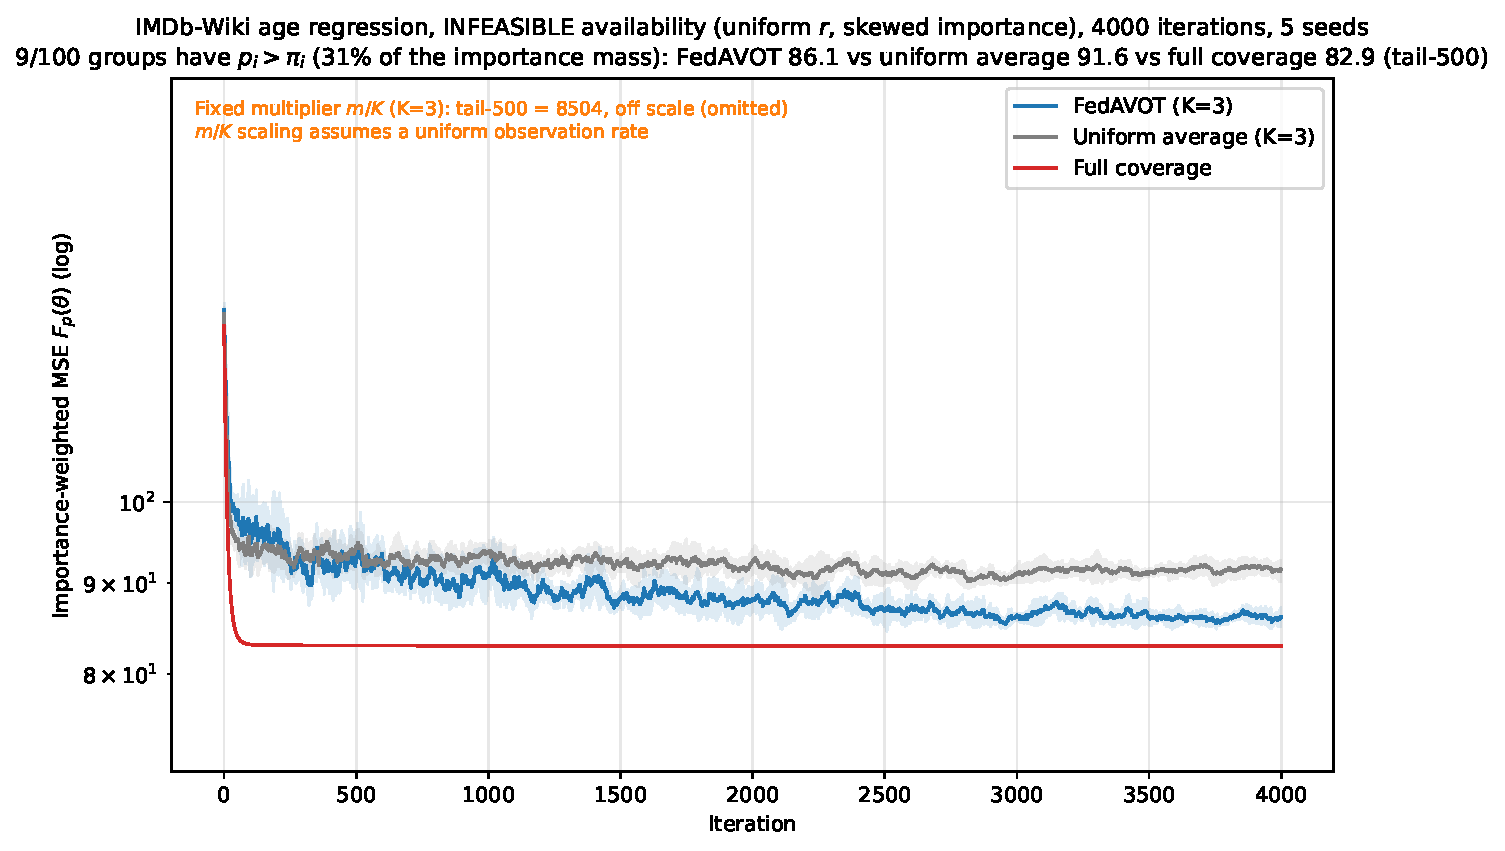
\includegraphics[width=\linewidth]{imdbwiki_infeasible_K3_4000rounds_decay.pdf}
  \caption{IMDb-Wiki age regression under uniform availability ($\beta=0$;
  $p_i \propto (m{+}1{-}i)^3$, $r$ uniform; $5$ seeds, shaded $\pm 1$ std).
  The cubic target is infeasible for $9$ groups holding $31\%$ of the
  importance mass, yet FedAVOT ($86.1$) recovers two thirds of the gap
  between the uniform average ($91.6$) and full coverage ($82.9$); the
  fixed-multiplier correction is unstable and off scale.}
  \label{fig:imdb-infeasible}
\end{figure}
\begin{figure}[t]
  \centering
  
\includegraphics[width=\linewidth]{imdbwiki_feasible_K3_4000rounds_decay.pdf}
  \caption{IMDb-Wiki under the aligned (feasible) availability regime
  ($r_i \propto m{+}1{-}i$). With $p_i \le \pi_i$ satisfied for all groups,
  FedAVOT ($84.3$) converges to within $1.3$ of the full-coverage objective
  ($82.9$) and below the uniform average ($86.4$); the fixed-multiplier
  correction diverges, as its fixed $m/K$ debiasing presumes a uniform
  observation rate.}
  \label{fig:imdb-feasible}
\end{figure}
\begin{figure*}[t]
  \centering
  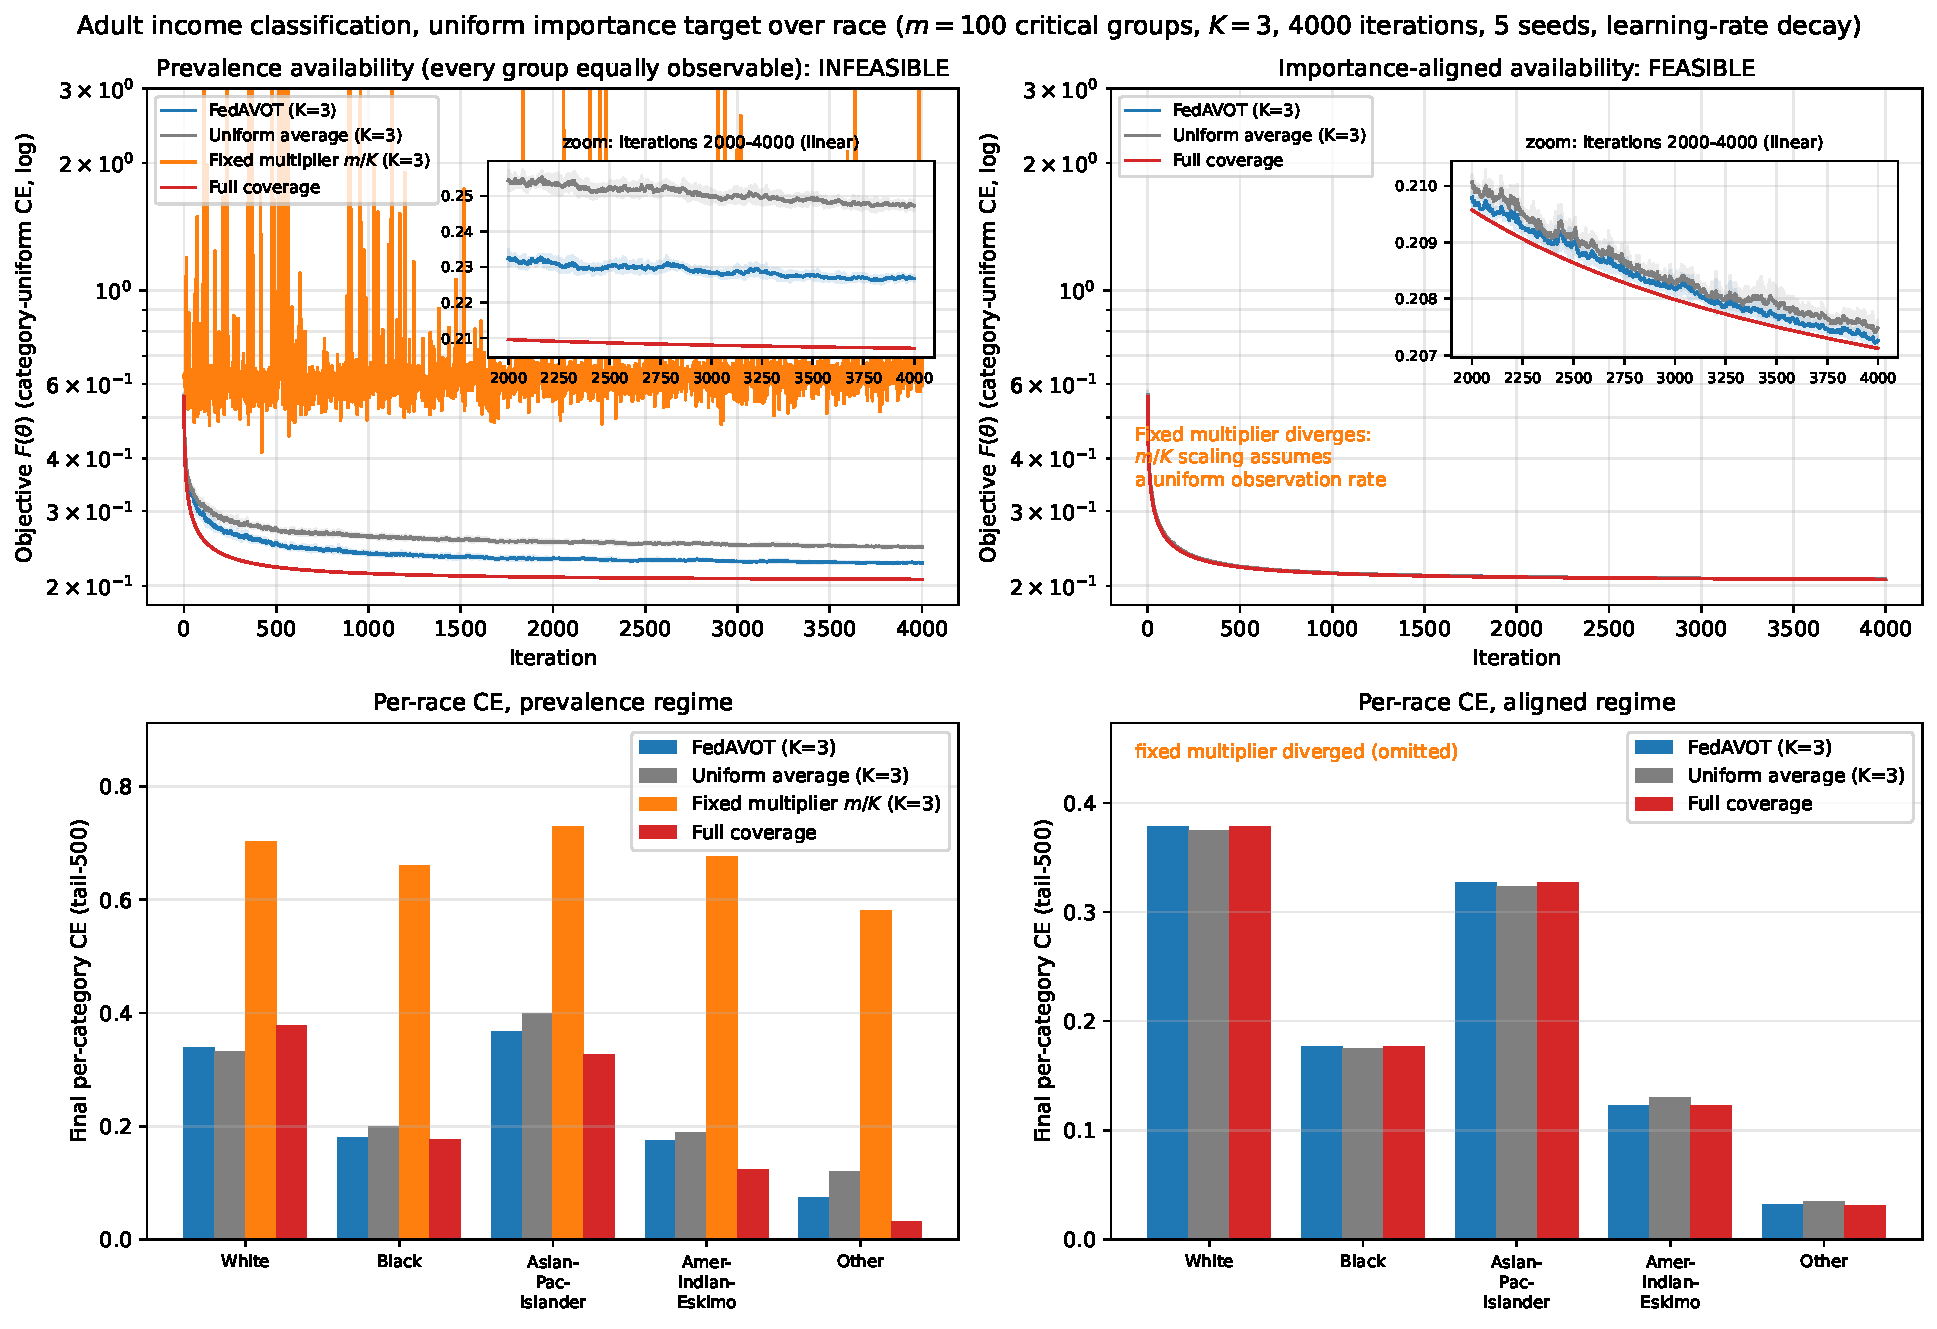
\includegraphics[width=0.88\textwidth]{adult_race_K3_4000rounds_decay.pdf}
  \caption{Adult income classification with a uniform importance target over
  race ($m=100$ groups, $K=3$, $4000$ iterations, $5$ seeds). Left column:
  prevalence availability (every group equally observable) makes the fairness
  target infeasible purely from category imbalance; FedAVOT ($0.227$) stays
  within $10\%$ of full coverage ($0.207$) and $8.5\%$ below the uniform
  average ($0.248$), while the fixed-multiplier correction is unstable, and
  the residual loss concentrates on the smallest race categories (bottom
  row). Right column: importance-aligned availability is feasible; FedAVOT
  and the uniform average both sit on top of full coverage and the
  fixed-multiplier correction diverges.}
  \label{fig:adult}
\end{figure*}
\begin{figure*}[t]
  \centering
  
\includegraphics[width=\textwidth]{fedavot_phase_boundary.pdf}
  \caption{Synthetic feasibility sweep. Left/center: loss trajectories in a
  feasible ($\alpha=0.5$) and an infeasible ($\alpha=3$) regime. Right:
  final loss versus the fraction of importance mass violating
  $p_i \le \pi_i$; FedAVOT's degradation relative to full coverage
  (annotated ratios) grows with the infeasible mass.}
  \label{fig:phase}
\end{figure*}
\begin{figure}[t]
  \centering
  
\includegraphics[width=\linewidth]{fedavot_mechanism.pdf}
  \caption{Mechanism of the failure. In the feasible regime ($\alpha=0.2$)
  Sinkhorn scaling matches the importance marginal to machine precision and
  every group receives its target weight; in the infeasible regime
  ($\alpha=3$) the row-marginal error stalls and high-importance groups are
  pinned at their inclusion-probability ceiling $\pi_i$, leaving $78\%$ of
  the importance mass undeliverable (the excess $\sum_i (p_i-\pi_i)_+$;
  the violating groups themselves hold ${\approx}87\%$ of the total
  importance mass, the figure quoted for the sweep).}
  \label{fig:mechanism}
\end{figure}
% ---------------------------------------------------------------- results prose
The uniform and aligned regimes bracket the feasibility condition
(Figs.~\ref{fig:imdb-infeasible} and~\ref{fig:imdb-feasible}). Under
uniform availability the transport problem is infeasible for $9$ of $100$
groups holding $31\%$ of the importance mass, and Sinkhorn scaling stalls
(row-marginal error ${\approx}9\times10^{-3}$ at termination). FedAVOT
nevertheless attains a final importance-weighted MSE of $86.06 \pm 0.21$
against $91.63 \pm 0.56$ for the uniform average and $82.95$ for full
coverage: it closes two thirds of the uniform average's excess over full
coverage, and the margin is ten seed standard deviations. The
fixed-multiplier correction is unstable here (tail mean $8.5\times10^{3}$),
since its $m/K$ scaling assumes that the per-group weight $(m/K)\,p_i$ is
bounded, which the cubic target violates. In the aligned regime the same
importance distribution becomes fully feasible, Sinkhorn converges
(row-marginal error ${\approx}5\times10^{-9}$), and FedAVOT attains
$84.28 \pm 0.15$ versus $86.37 \pm 0.34$ for the uniform average, within
$1.3$ of the full-coverage value. The fixed-multiplier correction
\emph{diverges} in this regime: under availability-aligned sampling the
realized aggregation weights exceed unity in expectation, exponentially
amplifying the iterates. FedAVOT is immune by construction, since each
column of $Y$ is a convex combination.
\paragraph{Real-Data Feasibility Sweep: the Floor Gap Predicts the Sign}
Table~\ref{tab:sweep} sweeps the availability skew $\beta$ on IMDb-Wiki.
Because the task is linear regression, the minimizer of the objective each
rule actually optimizes in expectation is available in closed form (the
\emph{floor}; see the bias validation below): FedAVOT minimizes
$F_{\hat{p}}$ with the stalled surrogate $\hat{p}$, while the uniform
average minimizes $F_{\tilde{p}}$ with $\tilde{p}_i = \pi_i/K$. The gap
between the two floors is $7.0$ at $\beta=0$ and shrinks monotonically to
$0.02$ at $\beta=3$, where both surrogates starve the same groups. The
measured margin of FedAVOT over the uniform average tracks this floor gap
at every $\beta$, and its sign flips exactly where the floors cross: FedAVOT
wins by $5.6$, $3.5$, $2.1$ and $0.6$ at $\beta \le 1.5$, ties at
$\beta=2$, and trails by $2.3$ in the mirrored regime. The floor gap is a
function of $(p,q,\mathcal{E})$ alone, so it can be computed before training
to decide whether transport reweighting will help. The step-size schedule is
what makes the bias visible: at a constant step size FedAVOT trails the
uniform average at every $\beta$ (e.g.\ $95.6$ versus $94.8$ at $\beta=0$
and $116.4$ versus $108.5$ at $\beta=3$), because its per-batch weights
concentrate mass on the few important groups present, which lowers the
effective batch size and raises the variance of the iterate; the decaying
schedule removes this variance term and exposes the bias that the transport
corrects.
\begin{table}[t]
  \centering\footnotesize\setlength{\tabcolsep}{3.5pt}
  \caption{IMDb-Wiki availability sweep, $r_i \propto i^{\beta}$, $5$ seeds,
  final importance-weighted MSE (full coverage: $82.9$). $F^{\dagger}$ are the
  closed-form floors, i.e.\ the minimizers of the objective each rule
  optimizes in expectation; $\Delta$ is the measured margin of FedAVOT over
  the uniform average, which follows the floor gap and changes sign where
  the floors meet.}
  \label{tab:sweep}
  \begin{tabular}{crrrrrr}
    \hline
    $\beta$ & inf.\ mass & $F^{\dagger}_{\mathrm{FedAVOT}}$ & $F^{\dagger}_{\mathrm{unif}}$ & FedAVOT & uniform & $\Delta$ \\
    \hline
    $0$   & $31\%$ & $83.4$  & $90.4$  & $86.1$  & $91.6$  & $+5.6$ \\
    $0.5$ & $59\%$ & $90.1$  & $95.8$  & $93.2$  & $96.7$  & $+3.5$ \\
    $1$   & $70\%$ & $95.3$  & $99.0$  & $97.9$  & $99.9$  & $+2.1$ \\
    $1.5$ & $77\%$ & $98.7$  & $101.2$ & $101.2$ & $101.8$ & $+0.6$ \\
    $2$   & $82\%$ & $101.4$ & $103.0$ & $103.8$ & $103.7$ & $0.0$ \\
    $3$   & $88\%$ & $105.9$ & $105.9$ & $108.4$ & $106.1$ & $-2.3$ \\
    \hline
  \end{tabular}
\end{table}
\paragraph{Results of the Synthetic Sweep}
The controlled study (Fig.~\ref{fig:phase}) confirms that feasibility (not
the aggregation rule) governs convergence. When the transport is feasible
FedAVOT tracks full coverage (final-loss ratio $1.01$ at $\alpha=0.5$
over $5000$ iterations), while its final loss degrades monotonically as the
infeasible importance mass grows, up to $8.4\times$ the full-coverage
loss at $\alpha=3$ (${\approx}87\%$ infeasible mass).
Fig.~\ref{fig:mechanism} exposes the mechanism: in the feasible regime the
row-marginal error decays to ${\sim}10^{-10}$ within $56$ Sinkhorn
iterations and the achieved group weights sit on the diagonal against their
targets, whereas in the infeasible regime the error stalls at
${\sim}8\times10^{-2}$ and every violating group is pinned at its inclusion
probability $\pi_i < p_i$; the undeliverable $78\%$ of the importance
mass accounts quantitatively for the loss floor observed in training.
\paragraph{Adult Results: Equal Availability Does Not Make a Fair Target Reachable}
The Adult experiment (Fig.~\ref{fig:adult}) transfers the same dichotomy
to a fairness setting. In the prevalence regime the transport is
infeasible for the five groups belonging to the three smallest race
categories ($60\%$ of the importance mass; Sinkhorn row-marginal error
stalls at ${\approx}1.7\times10^{-1}$): FedAVOT attains a category-uniform
cross-entropy of $0.2269 \pm 0.0005$ versus $0.2479 \pm 0.0009$ for the
uniform average, $0.670 \pm 0.031$ for the fixed-multiplier correction, and
$0.2073$ for full coverage, i.e., within $10\%$ of the full-coverage
objective and $8.5\%$ below the uniform average; but the unrecoverable loss
concentrates precisely on the categories the uniform target was meant to
protect (final per-category cross-entropy $0.175$ versus full coverage's
$0.123$ for Amer-Indian-Eskimo, $0.073$ versus $0.031$ for Other, with the
uniform average worse still at $0.189$ and $0.119$). Along the
interpolating family $r \propto p^{\beta}$ FedAVOT improves on the uniform
average at every $\beta$ (margins $0.021$, $0.018$, $0.013$, $0.005$,
$0.0002$ for $\beta = 0, 0.25, 0.5, 0.75, 1$), and once the target is
feasible ($\beta \ge 0.5$) it matches full coverage to three decimals while
the uniform average remains $2$--$6\%$ above it. In the aligned regime
($\beta=1$, row error ${\approx}3\times10^{-8}$) FedAVOT reaches
$0.2075 \pm 0.0001$, on top of the full-coverage value, and the
fixed-multiplier correction again diverges. Equal observability for every
group is therefore not sufficient for fairness: when category sizes are
imbalanced, a category-uniform objective violates the feasibility condition,
and the deficit lands on the protected minorities.
\paragraph{Risk-Averse Aggregation Does Not Substitute for Alignment}
A natural alternative to per-batch alignment is to reweight \emph{across}
iterations by risk aversion, as in the CVaR-based scheme of~\cite{theodoropoulos2023cvar}, which amplifies the step of any batch whose loss exceeds a running threshold (tail level $\alpha$, amplification $\gamma$). We run this scheme on top of both the uniform average and FedAVOT over a $10\times10$ grid of $(\alpha,\gamma)\in\{0.1,\dots,1\}^2$ on the four settings above ($5$ seeds each). On the importance-weighted objective, risk aversion never helps: in every setting the best grid point of either combination is the risk-neutral corner $\gamma=1$, at which the scheme reduces to its base rule, and the most aggressive corner $(\alpha,\gamma)=(0.1,0.1)$ costs $14$--$25\%$ on the objective. Its effect is confined to the worst-category loss on Adult in the prevalence regime, where FedAVOT combined with CVaR at $(\alpha,\gamma)=(0.2,0.7)$ lowers the worst race category's cross-entropy from $0.368$ to $0.362$, against $0.390$ for the uniform average with CVaR ($0.399$ without) and $0.379$ for full coverage, at a cost of $0.008$ ($3.5\%$) on the overall objective. Alignment and risk aversion thus act on different axes, within and across batches respectively, and only the former changes which objective is reachable.
\paragraph{Empirical Validation of the Infeasibility Bound}
All runs in this section fit $T$ by plain masked Sinkhorn scaling
(Algorithm~\ref{alg:sinkhorn}), without marginal relaxation ($\lambda = 0$
in \eqref{eq:general-reg-failure}). In the infeasible regimes the iteration
stalls, and the returned plan delivers exactly the surrogate marginal
$\hat{p} = T\mathbf{1}$ of \eqref{eq:phat-failure}: because the column
marginals match $q$ at termination, the expected aggregation weight of group
$i$ at each iteration equals $\hat{p}_i$, so training minimizes the surrogate
objective $F_{\hat{p}}$ and the bias term of \eqref{eq:infeasible-rate}
becomes directly measurable. In the mirrored IMDb-Wiki regime ($\beta=3$,
constant step size $\eta_\theta$ for this paragraph) the stalled
marginal truncates the target at the inclusion-probability ceiling,
$\hat{p}_i \approx \min(p_i, \pi_i)$ up to renormalization (maximum
deviation $0.023$), yielding $\|p - \hat{p}\|_1 = 1.58$ of a maximum
possible $2$. Since the task is linear regression, the minimizers
$\theta^\star$ of $F_p$ and $\theta^\dagger$ of $F_{\hat{p}}$ are available
in closed form, which isolates the bias of \eqref{eq:infeasible-rate} from
optimization error: $F_p(\theta^\star) = 82.9$, matching the observed
full-coverage plateau ($83.07$), whereas $F_p(\theta^\dagger) =
105.9$. The marginal shift alone therefore costs $22.9$, the bulk of
FedAVOT's measured excess of $33.3$ over full coverage; the remainder
is consistent with the sampling variance of $K=3$ groups per batch and
$H=5$ local steps at a fixed step size. The uniform average admits the
same analysis with $\tilde{p}_i = \pi_i/K$ in place of $\hat{p}$, and its
floor is also $105.9$: in this regime the two surrogates starve the same
groups, so the rules share a floor and the lower-variance uniform average
wins ($108.5$ versus $116.4$ at a fixed step size), whereas at $\beta=0$
the floors separate by $7.0$ (Table~\ref{tab:sweep}) and FedAVOT wins. The
realized bias equals its exact expression $|F_p(\theta^\dagger) - F_{\hat{p}}(\theta^\dagger)| =
|(p - \hat{p})^\top L(\theta^\dagger)| = 30.7$, where $L(\theta)$ collects
the per-group expected losses; the worst-case form $2B\|p - \hat{p}\|_1$ of
\eqref{eq:infeasible-rate} holds but is conservative here, since any
uniform bound satisfies $B \ge \max_i L_i(\theta^\dagger) \approx 454$.
The same quantity organizes the synthetic sweep: $\|p - \hat{p}\|_1$ grows
from $0.08$ at $\alpha = 0.5$ to $1.57$ at $\alpha = 3$, tracking the
monotone degradation of Fig.~\ref{fig:phase}.
Finally, we run the marginal-penalized family
\eqref{eq:general-reg-failure} itself (KL penalty, $\varepsilon = 1$) on
the mirrored regime, sweeping $\lambda$ from $0$ to $\infty$; the two
endpoints are, respectively, uniform averaging over the drawn subset and
the plain masked IPFP above. Under this severe infeasibility $\lambda$ has
almost no purchase on the bias: $\|p - \hat{p}(\lambda)\|_1$ moves only
from $1.74$ to $1.58$ and the closed-form floor stays within
$[104.0,\,105.9]$, yet the measured loss increases from $108.3 \pm 0.8$
(at $\lambda = 1/4$) to $116.5 \pm 0.7$ (at $\lambda = \infty$): stronger
adherence penalties produce more extreme per-batch weights, buying
variance rather than reachability. When infeasibility is severe, the
regularization path of Section~\ref{subsec:infeasible} is therefore best
read as a variance--bias tradeoff in which small $\lambda$ is preferable.
\bibliographystyle{plain}
\bibliography{refrences}
\end{document}